
%%% Local Variables:
%%% mode: latex
%%% TeX-master: t
%%% End:

\documentclass{beamer}

\usetheme{boxes}
\usepackage[utf8]{inputenc}
\usepackage{tikz}
\usetikzlibrary{calc,shapes.multipart,chains,arrows}

\begin{document}

\begin{frame}

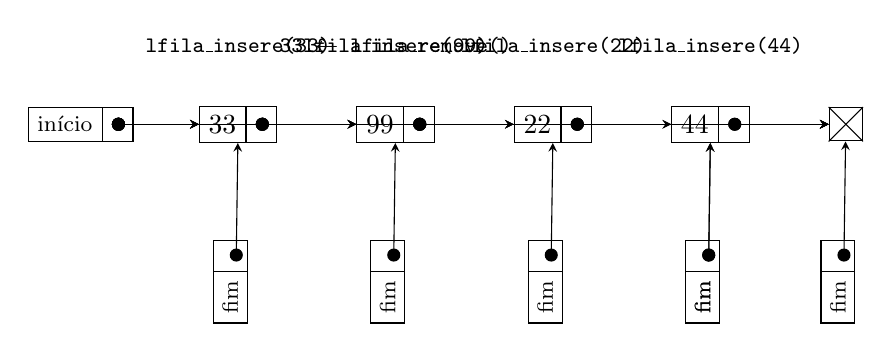
\begin{tikzpicture}
\def\shift{2cm}

\tikzset{
    list/.style={rectangle split, rectangle split parts=2,
    draw, rectangle split horizontal}, 
    >=stealth, start chain
}

  \node[list,on chain] (INI) {\footnotesize início};
  \node<2-5>[list,on chain] (A) [right of=INI] {33};
  \node<3->[list,on chain] (B) [right of=A]   {99};
  \node<4->[list,on chain]  (C) [right of=B]    {22};
  \node<5->[list,on chain]  (D) [right of=C]    {44};

  \node[on chain,draw,inner sep=6pt] (NULL) {};
  \draw (NULL.north east) -- (NULL.south west);
  \draw (NULL.north west) -- (NULL.south east);


  \def\tail{NULL}
  \node<1>[list,rotate=90] (END) [left of=\tail, xshift=-.5*\shift,yshift=.05*\shift] {\footnotesize fim};

  %START
  \draw<1>[*->] let \p1 = (INI.two), \p2 = (INI.center) in (\x1,\y2)  -- (NULL);
  \draw<1>[*->] (END.two) -- (NULL) ;

  %QUEUE 33
  \def\tail{A}
  \node<2> [above of=\tail] {{\tt\footnotesize lfila\_insere(33)}};
  \draw<2>[*->] let \p1 = (INI.two), \p2 = (INI.center) in (\x1,\y2)  -- (A);
  \draw<2>[*->] let \p1 = (A.two), \p2 = (A.center) in (\x1,\y2)  -- (NULL);
  \node<2>[list,rotate=90] (END) [left of=\tail, xshift=-.5*\shift,yshift=.05*\shift] {\footnotesize fim};
  \draw<2>[*->] (END.two) -- (\tail) ;

  %QUEUE 99
  \def\tail{B}
  \node<3> [above of=\tail] {{\tt\footnotesize lfila\_insere(99)}};
  \draw<3>[*->] let \p1 = (INI.two), \p2 = (INI.center) in (\x1,\y2)  -- (A);
  \draw<3>[*->] let \p1 = (A.two), \p2 = (A.center) in (\x1,\y2) -- (B);
  \draw<3>[*->] let \p1 = (B.two), \p2 = (B.center) in (\x1,\y2)  -- (NULL);
  \node<3>[list,rotate=90] (END) [left of=\tail, xshift=-.5*\shift,yshift=.05*\shift] {\footnotesize fim};
  \draw<3>[*->] (END.two) -- (\tail) ;


  %QUEUE 22
  \def\tail{C}
  \node<4> [above of=\tail] {{\tt\footnotesize lfila\_insere(22)}};
  \draw<4>[*->] let \p1 = (INI.two), \p2 = (INI.center) in (\x1,\y2)  -- (A);
  \draw<4>[*->] let \p1 = (A.two), \p2 = (A.center) in (\x1,\y2) -- (B);
  \draw<4>[*->] let \p1 = (B.two), \p2 = (B.center) in (\x1,\y2)  -- (C);
  \draw<4>[*->] let \p1 = (C.two), \p2 = (C.center) in (\x1,\y2)  -- (NULL);
  \node<4>[list,rotate=90] (END) [left of=\tail, xshift=-.5*\shift,yshift=.05*\shift] {\footnotesize fim};
  \draw<4>[*->] (END.two) -- (\tail) ;

  %QUEUE 22
  \def\tail{D}
  \node<5> [above of=\tail] {{\tt\footnotesize lfila\_insere(44)}};
  \draw<5>[*->] let \p1 = (INI.two), \p2 = (INI.center) in (\x1,\y2)  -- (A);
  \draw<5>[*->] let \p1 = (A.two), \p2 = (A.center) in (\x1,\y2) -- (B);
  \draw<5>[*->] let \p1 = (B.two), \p2 = (B.center) in (\x1,\y2)  -- (C);
  \draw<5>[*->] let \p1 = (C.two), \p2 = (C.center) in (\x1,\y2)  -- (D);
  \draw<5>[*->] let \p1 = (D.two), \p2 = (D.center) in (\x1,\y2)  -- (NULL);
  \node<5>[list,rotate=90] (END) [left of=\tail, xshift=-.5*\shift,yshift=.05*\shift] {\footnotesize fim};
  \draw<5>[*->] (END.two) -- (\tail) ;

  %ENQUEUE
  \def\tail{D}
  \node<6> [above of=B] {{\tt\footnotesize 33 $\leftarrow$ lfila\_remove()}};
  \draw<6>[*->] let \p1 = (INI.two), \p2 = (INI.center) in (\x1,\y2)  -- (B);
  \draw<6>[*->] let \p1 = (B.two), \p2 = (B.center) in (\x1,\y2) -- (C);
  \draw<6>[*->] let \p1 = (C.two), \p2 = (C.center) in (\x1,\y2)  -- (D);
  \draw<6>[*->] let \p1 = (D.two), \p2 = (D.center) in (\x1,\y2)  -- (NULL);
  \node<6>[list,rotate=90] (END) [left of=\tail, xshift=-.5*\shift,yshift=.05*\shift] {\footnotesize fim};
  \draw<6>[*->] (END.two) -- (\tail) ;


\end{tikzpicture}

\end{frame}

\end{document}